\section{Use Cases}

\subsection{Actors}

\subsection{Use case diagrams}
See figure \ref{fig:usecase} at page \pageref{fig:usecase}.

\begin{figure}
\begin{center}
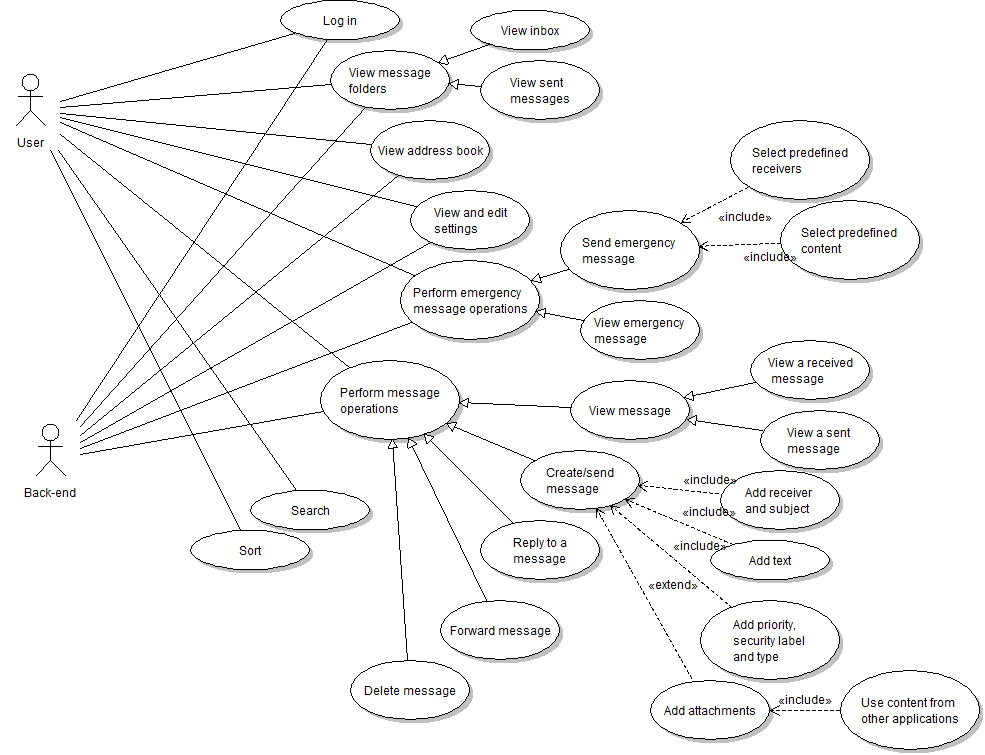
\includegraphics[width=\textwidth]{kpro-use-case}
\caption{Use case diagram} \label{fig:usecase}
\end{center}
\end{figure}

\subsection{Textual use cases}
Each of the use cases are describe below, so that the use case diagram will be easier to understand. See table \ref{tab:viewmessages} - \ref{} starting at page \pageref{tab:viewmessages} to take a closer look at the use cases.

\begin{table}
\begin{tabular}{p{3cm}|p{12cm}}
Element & Description \\ \hline
Use case name & View messages \\
Goal & View received and sent messages \\
Summary &The user would like to view received and sent messages \\
Preconditions &
\begin{enumerate}
\item{}The application is running.
\item{}The user is logged in.
\end{enumerate} \\ \hline
Flow of Events &
\begin{enumerate}
\item{}The user selects a message from either the sent, inbox or outbox messages.
\item{}Message is showed to user.
\end{enumerate} \\ \hline
Exceptions & There are no existing messages.
\end{tabular}
\caption{View messages textual use case} \label{tab:viewmessages}
\end{table}

\begin{table}
\begin{tabular}{p{3cm}|p{12cm}}
Element & Description \\ \hline
Use case name & Create message \\
Goal & User creates a complete message \\
Summary &The user would like to create a message with a subject and text. The user would also like to set the priority, security label and type of the message as well as being able to add an attachment. \\
Preconditions &
\begin{enumerate}
\item{}The application is running.
\item{}The user is logged in.
\end{enumerate} \\ \hline
Flow of Events &
\begin{enumerate}
\item{}User selects new message.
\item{}The user adds the recipient(s) and subject to the message.
\item{}The user sets the priority, security label and type.
\item{}The user adds attachments if needed.
\end{enumerate} \\ \hline
Exceptions & The user does not set priority, security label and type and default values are set.
\end{tabular}
\caption{Create message textual use case} \label{tab:createmessage}
\end{table}

\begin{table}
\begin{tabular}{p{3cm}|p{12cm}}
Element & Description \\ \hline
Use case name & View and interact with address book \\
Goal & User can view and interact with the address book \\
Summary &The user enters the address book and is able to view, add, edit and delete contacts. \\
Preconditions &
\begin{enumerate}
\item{}The application is running.
\item{}The user is logged in.
\end{enumerate} \\ \hline
Flow of Events &
\begin{enumerate}
\item{}User selects address book.
\item{}User either adds a new contact or selects an existing one.
\item{}If the user selects an existing contact, he can either edit that contact or delete it.
\end{enumerate} \\ \hline
Exceptions & ??
\end{tabular}
\caption{View and interact textual use case} \label{tab:viewandinteract}
\end{table}